\chapter{Introduction}
\label{cha:intro}

% Important: you have to switch to arabic numbering here!
\pagenumbering{arabic}

%\begin{itemize}
%\item Background / Context of the thesis 
%\item If applicable: describe the project the thesis is related to (e.g., CoCar)
%\item Problem / Motivation
%\item Goals of the thesis
%\item For final thesis document: outline of the document
%\end{itemize}

%This is an example for a citation \cite{DBLP:journals/jods/KenscheQCJ07}.

With the development of new technology and technology oriented devices now the data produces continuosly in a heterogeneous structure in every single second. According to statistics of youtube, in every minute hours of video uploaded to YouTube is 300 hours equivalent to watch \cite{p301}. Recently, sensors and Internet of Things devices produce data in a continuous fashion with each and every single second. As a consequece, we are now having a wide variety of large, complex, high-dimensional dataset. Data scientist and researchers are doing research on finding optimum way of collecting data, storing data, analysing data, proposed new algorithm for data mining, finding training methods to train the data, visualizing data and many more. Due to the various characteristics of the data in respect of size, structure, format there has been always challenging issue arises in the existing field and also new research domain being created.\\\\
We are living in the world called "Big Data". These Big Data have diversified sources such as images, videos,  different social sites activities like post status, comments etc. Moreover now-a-days a lot of data is generated through sensors applied in different fields, GPS signals and many more \cite{p302}. The term "Big Data" is first mentioned on the IEEE 8th conference on visualisation in year 1997 \cite{p303}. However, since 2011 the interest in big data area had been increased exponentially \cite{p304}. The word "Big" means significance, complexity, challenge, quantification.\\\\
There are many definition for the Big Data but unfortunately there is no exact established definition throughout the whole world wide. The most used one is from Gartner report \cite{p305}. According to that, data those can be termed the "three Vs":  volume,variety and velocity are known as big data. Volume means the significant amount of data produces from the source. Data are produced in a structured, semi-structured or sometimes non-structured way which defined by the term variety. Velocity is the rate at which data is being produced. Later, two new addidational "V"'s are added known as Veracity and Value. Veracity is for the trustworthiness of the data and value determines the business value add in the dataset.\\\\
Data can be modelled based on some characteristics. Traditionally, data is modelled as persistent relationships and store into database management system. From the system, data can be accessed and analysed based on the requirements. But recently a new class of data intensive application evolved where application does not follow the traditional system rather considered as transient data streams. Examples of such application fields include financial applications, web page visits, network monitoring, security, telecommunication data management, sensor network  and many more \cite{p306}. In data streams, data produce continously in multiple structured with the flow of the time. Datas are unbounded and unpredictable as well. Due to having this unique characteristics; a new approach is required to capture, storage, transformation data.\\\\
In many application field real time analysis is very much important. For example, in medical domain there are many diagnostic data has been generated from different machine where doctors need to analyse the data and take decision in real time. In stock market, price are continuously changing as time changes and the traders need to analyse those data and take decision of doing transaction in real time. The same type of real-time analysis is also needed  with the sensor data attached with the internet of devices or the meteorological data and space data.\\\\
In present world, each data set has a huge number of features or dimensions. In general, the features are those which help to describe the data. These are called as "High-Dimensional Data" and in almost every fields of study starting from meterology to economics field now data are high dimensional. The computational complexity and storage complexity increases with the increament of the dimensions. Moreover, if a data is high dimensional then it is also difficult for the human being to reflect their intuitions to percept the knowledge from the data. Although each feature has the important information of the data set but still we can compare among the features based on the important information and skip the less feature one and this process is known as dimensionality reduction.\\\\
The concept of using pictures to understand data has been around for the centuries and the process to present data in forms of pictures or graphs is known as data visualization. With the help of visualisation it is easy to get the inner meaning of the data. Though earlier visulaization is only used for the communication but now the visualization is also helpful to achieve the inner meanings of the data. It helps us to analyse the data and present in form of patterns, trends, gaps and outliers. It also helps us to compare, make correlations among the data. One of the most important benefit of visualisation is that it encompasses various data set quickly, effectively and efficiently. Scientifically the effectiveness of data visualization is to maintain a proper balance between perception and cognition through visualisation.\\\\
In last few decades, huge number of efforts have been introduced for data visualization. Many tools have already been published for the effective visualization but still it is one of the open research field for visualization researcher to build an effective tool for high dimensional data visualization. Some of the most conventional visualization tools are Histogram, x-y plots, line plots, scatter plots, Venn diagram, pie charts etc. These visualization method are not suitable enough for high Dimensional Data \cite{pf01}. Though some new methods like Tree map, paralel coordinates, Heat Map are emerged as extensions to the convolutional method but still these techniques are far from the target and also suffer because of high dimensions. Due to the lack of proper high dimensional data visualizaiton tool one of the prominent way is to reduce the dimensions efficiently to preseve information as much as possible and then visulaize the result with any of the extending visualization tool.\\\\
Though High Dimensional static data have been studied out for the last few decade but still there is no far research has been carried out for the dynamic or streaming data. There are many algorithms for high dimensional data which works fine for the static data set but the performance deteriotes for the streaming one. Moreover, the dimensionality reduction method is not evaluated from visualization perspective in streaming area. In this thesis, this problem is identified and will try to provide a solution for dimensionality reduction in streaming data and also evaluate through visualisation technique.    

\section{Motivation}
Due to the growth of streaming data it is now demand of the some application domain to analyse the data and present data to the end user in quick response. For example, in stock market data produce continuously about telling the price, volume of the stock etc; if a system can analyse the pattern of the data, find correlation among the features and present them intuitively to the end users then users will be able to take a quick decision to buy the perfect stock at that time and do profit more.\\\\
The necessity of visulaization in this kind of scenario opens up the challenge for the researcher to present the user friendly, intuitive, interactive, easily understandable visulisation to the end user. There are three main transforamtion steps to achieve such a effective visualization \cite{pf03}. These are: 
\begin{enumerate}
	\item Data transformation
	\item Visual mapping
	\item View transformation
\end{enumerate}
Data transformation is the process of transforming source data to suitable vesrion of the data for carrying further process. There are many ways to transform data and Dimensionality reduction is one of them. Moreover, dimensionality reduction is not only the effective for the visualization but also helpful to build many effective data model. It is also helpful for any learning algorithm.\\\\
There are two different ways to reduce dimensions from the original dataset. The reduction can be done either by selecting significant features and form a subset of the original set. The other way to reduce it by transforming dimension in order to get a new one or reduced set of dimensions. The first one is called the Feature Selection which is greedy in nature where the later one is known as Feature Extraction. Due to the nature of Feature Selection it is always a challenge an optimal solution or the subset based on some defined criteria. Orthogonal Centroid Algorithm is a Feature Selection algorithm.\\\\
Feature Extraction algorithm aim to extract features by projecting high-dimensional space into lower dimensional space using algebraic expression. The feature extraction algorithm can be further divided into linear projection and non-linear projection. Linear Discriminant Analysis (LDA), Maximum Margin Classification (MMC) \& Principle Component Analysis (PCA) are linear feature extraction algorithm \cite{thesis1} where non-linear algorithm are kernel PCA, graph-kernel PCA etc.\\\\
The conventional dimensionality reduction algorithm use Gaussian Maximum Likelihood estimation which involves different matrices like covariant matrix, scatter matrix which have time \& space complexity of \textit{O($n^{2}$)} or \textit{O($n^{3}$)}. The complexity can be tolerable if the data size is small but if the data sample is more than 20000 then this method does not perform well \cite{p307}. Due to the high mathematical computation it is not suitable to use those methods on streaming data specially in real time analysis field. The time increased rapidly for streaming data because everytime new data comes it starts from the scratch.\\\\
One of the solution is to propose incremental version of feature extraction algorithm. The term "incremental" means learning from new data without forgetting the prior knowledge. In this mechanism, a system must acquire knowledge from the past data without keeping the original data and also ready to handle the new data \cite{p316}.Incremental Principle Component Analysis(IPCA) \cite{thesis4}, Incremental Linear Discriminant Analysis \cite{1thesis2}, Candid Covariance-free incremental principle component analysis \cite{thesis5}, Incremental Dimension Reduction via QR decomposition \cite{thesis2} etc. The major drawback is still the involvement of numerical transformation which performs very poor where there is a lot of data \& dimensions. The details of each algorithm will be covered on the related work section.\\\\
In all of the incremental algorithm researchers use static data sets. They divide the data set into two portions where first portion they used to calculate all the mathematical computation and remember values irrespective of the dataset and later they used the remaining portion to update those values incrementally and see the final output of the algorithm. In our thesis, we will use time based streaming data having a fixed time window which is unpredictable in nature and also data will not available after the time pass. The existing use of data set is controlled by the user and also continuous update of visualization is interrupted. Moreover, the performance of any kind of incremental dimensionality reduction is not evaluated through visualization perspective.\\\\
Though dimensionality reduction has many advantages but it has some demerits too. The main drawback is the possibility of information loss. It is undoubtedly true that when we left of one dimension that means we have the trade off of loosing some data but in some cases we have lost the important information. The essential idea of dimensionality reduction is to preserve the instrinsic meaning of the data by keeping similar data points close and maintaining a distance among dissimilarity data. Researchers is now also looking for different approaches to get the same or better visualisation as ouput without doing information loss. One of them is reordering the columns based on similarities. Djuric et.all proposed an algorithm based on the reordering approaches in their paper  \cite{1thesis3}.The details will be covered in the "Entropy Minimisation ordering" of the related work section.
\section{Goals of the thesis} 
The aim of this thesis is to develop an effective visualization framework for Stream data. In this framework, we can select the high dimensional datasets from different domains and reduce the dimensions through dimensionality reduction algorithm. For dimensionality reduction we will use the incremental version of traditional dimensionality reduction algorithm known as Linear Discriminant Analysis. The another prime concern will be regarding the information loss due to the dimensionality reduction. Our framework will be evaluated regarding the information loss and also some more evaluation criteria. The visulaisation will be presented to the end user through HeatMap; one of the most used prominent tool for high dimensional data visualization technique. 
\begin{figure}[htbp]
	% center the image.
	\centering
	
	% include a png file. Adapt size to 0.5 * textwidth and retain aspect ratio (!)
	\resizebox{\textwidth}{!}{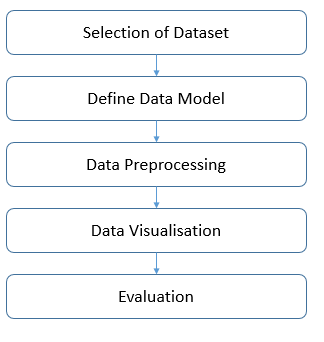
\includegraphics{Thesis_Goal.png}}
	
	\caption{Thesis Goals}
	\label{fig:labelOfMyFigure2}
\end{figure}
\subsection{Selection of Dataset}
In this thesis, we are looking for the high dimensional data set.There is no fixed threshold number of the dimension what can be termed as high but while we look for the data set we considered from visualisation perspective and ensure data set are high dimensional. If required we can convert the batch data to streaming data using any kind of state on art tool.
\subsection{Define Data Model}
The main difference between static data and streaming data is in static data we can save data into the disk and access that whenever we need that for any purpose but in streaming data the situation is not the same. In streaming data hence velocity of the data is huge so we can not save the data rather we need to do operations with the flow of data. Sliding window structure means we will divide the data in a block and only have access for once; there is no scope of viewing the data for the second time. The block can be done based on the time interval.
\subsection{Data Preprocessing}
Data preprocessing includes a lot of steps to be done before using the data. We will only focus on dimensionality reduction in this thesis and this is the core part of the thesis. There are many algorithms has been developed by researchers regarding Linear Discriminant Analysis and all of them either use the scatter matrix or QR decomposition under the big picture. Recently, one algorithm use Cholesky-decomposition to implement Linear Discriminant Analysis which is comparatively faster than others in theory but there is no open source of that code. Moreover, the algorithm is used for batch data set in an incremental way but we will directly imply the algorithm on stream data.
\subsection{Visualization}
Visualization is the beginning of the output section of the thesis.There are many state-on-art visualization techniques for visualize high dimensional data. We will visualize the output of the framework through one of the common procedure known as Heatmap.
\subsection{Evaluation}
There are basically two ways to evaluate the system. One is known as the quantitative evaluation and the other is qualitative evaluation. In Quantitative evaluation we define the metrics for example calculating the entropy or the matrix reordering quantitatively. Qualitative evaluation is the evaluation for example after showing the visualization by deciding which one is more informative. This can be done by doing user studies or selecting streaming data from different fields.\\\\
In our thesis we will follow the qualitative evaluation part by calculating different kind of matrices after getting the reduced dimensional data.\\\\
The remaining part of this paper is organized in the following manner: Section 2 will decribe the related work about dimensionality reduction, it will be followed by the solution of the thesis. Section 4 is for the evaluation and last section is the timeplan of the thesis. 


%\section{Figures}

%Use vector graphics wherever possible and avoid bitmap images. Do not
%use JPG at all (they are often blurred because of the compression). If
%you have to include a bitmap graphics, use the PNG format. If you have
%to use a JPG (as in the case for the logos on the title page), make sure
%that these are images with high resolution and high quality.
%\pdfcomment{pdfcomment is a useful package to put annotations like this one into the text.}

%The preferred way to create a PDF image to be used in LaTeX is the following:
%\begin{enumerate}
%\item Do the image with your favorite graphics program (Powerpoint works well for many cases).
%\item Print/Save the image as a PDF file (Acrobat Professional might be required, but
%there also Open Source solutions, e.g. FreePDF)
%\item Crop the image file and remove white margins.
%\item Include it in LaTeX as in this example.
%\end{enumerate}

%How to refer to images:
%Figure \ref{fig:labelOfFigure1} shows something from \cite{AfratiPODS2002}
%whereas figure \ref{fig:labelOfNextFigure} is about \cite{LenzeriniPODS2002}.

%If your image is not your own and taken from another source, cite the source
%also in the caption.

% priority where to place the figure: here, top, bottom, page
%\begin{figure}[htbp]
  % center the image.
 % \centering

  % include a png file. Adapt size to 0.5 * textwidth and retain aspect ratio (!)
 % \resizebox{\textwidth}{!}{
\includegraphics{Figure1.png}}

 % \caption{The text under the figure \cite{AfratiPODS2002}}
 % \label{fig:labelOfFigure1}
%\end{figure}


%\begin{figure}[htbp]
  %\centering
  % Include a pdf file but make it a little smaller than the textwidth
 % 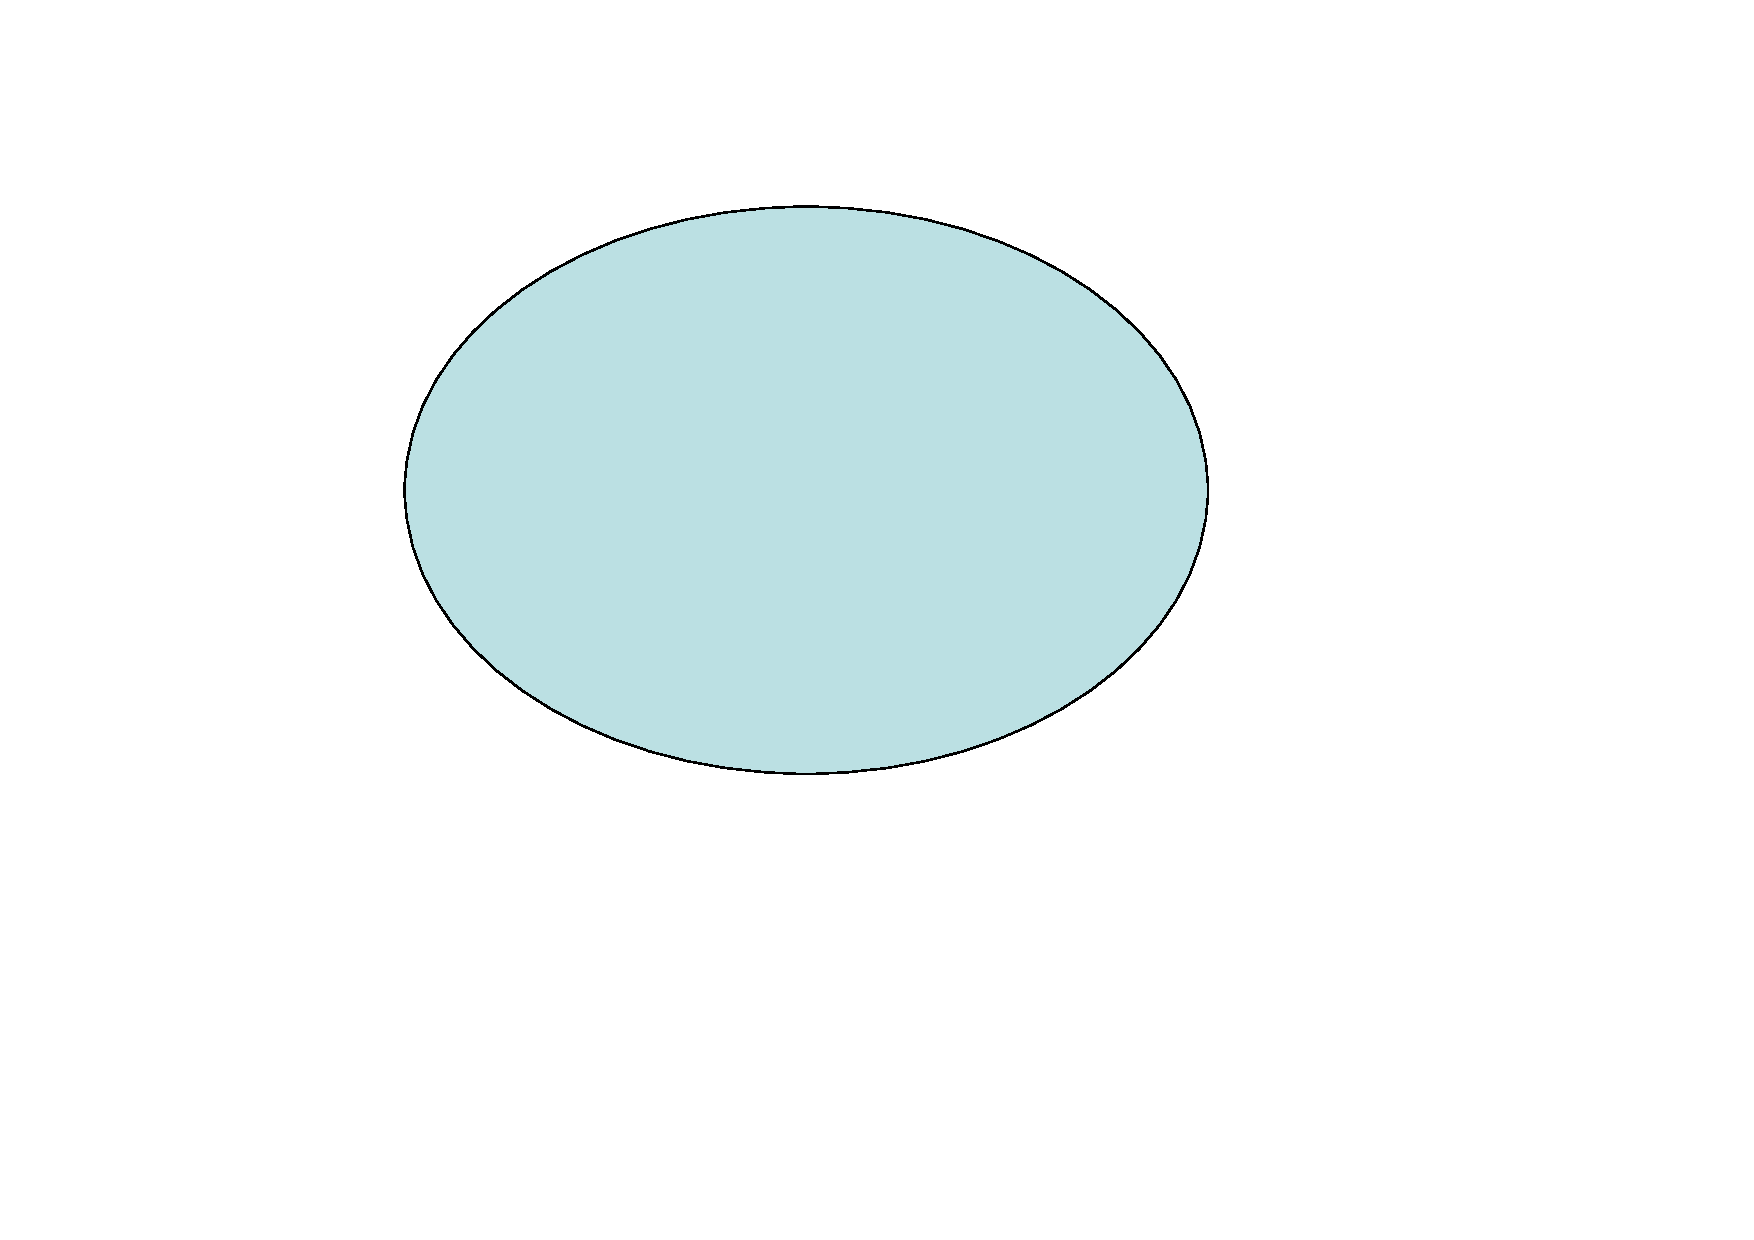
\includegraphics[width=0.5\textwidth]{Figure2.pdf}
  % Use EPS if you cannot create PDF files
  % (See http://www.wmf2eps.de.vu/ for creating eps files from powerpoint figures)
 % \caption{Another text under this figure \cite{LenzeriniPODS2002}}
 % \label{fig:labelOfNextFigure}
%\end{figure}

